\documentclass[a4paper,11pt]{article}

% --- Packages de base ---
\usepackage[utf8]{inputenc}
\usepackage[T1]{fontenc}
\usepackage[french]{babel}
\usepackage{graphicx}      % Pour inclure des images
\usepackage{amsmath, amssymb}
\usepackage{hyperref}      % Liens cliquables
\usepackage{geometry}      % Marges
\usepackage{float}         % Contrôle du placement des figures
\usepackage{caption}       % Légendes personnalisées
\usepackage{subcaption}    % Sous-figures
\usepackage{xcolor}        % Couleurs
\usepackage{fancyhdr}      % En-têtes et pieds de page
\usepackage{enumitem}      % Listes personnalisées

% --- Mise en page ---
\geometry{margin=2.5cm}
\setlength{\parskip}{0.7em}
\setlength{\parindent}{0pt}

% --- Infos du titre ---
\title{\textbf{Rapport intermédiaire - IMA}\\ \smallskip \large Enleveur de brume}
\author{Xu Boyang \\ Senart Mathieu}
\date{\today}


\begin{document}
\maketitle
\begin{large}
\textbf{Rappel de l'article :}
\end{large}
\\[1em]
Il s'agit de travailler sur le principe de l'enleveur de brume (dehazer) en suivant l'article de recherche de K. He, J. Sun et X. Tang, qui se base sur la supposition qu'il existe toujours pixels dont une de ses composantes rouge, verte ou bleu quelque soit le patch qu'on découpe sur une image.
\\[1em]
\begin{large}
\textbf{Progression :}
\end{large}
\\[1em]
Le papier a été implémenté de bout en bout : le \textit{dark channel} est calculé, la lumière ambiante en est déduite ainsi que la transmission. la technique de \textit{soft matting} comme recommandée par le papier a été aussi appliquée pour retrouver l'image sans brume.
\\[1em]
\begin{large}
\textbf{Résultats :}
\end{large}
\\[1em]
Nous avons vérifié le programme sur les images de la thèse. En voici les résultats :
\begin{figure}[H]
    \centering
    % Première image
    \begin{subfigure}[b]{0.27\textwidth}
        \centering
        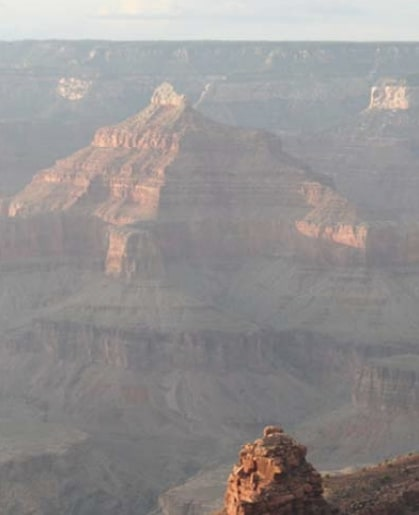
\includegraphics[width=\textwidth]{../hazed_images/4.jpg}
        \caption{{\scriptsize image enbrumée venant de la thèse}}
        \label{fig:image1}
    \end{subfigure}
    % Deuxième image
    \begin{subfigure}[b]{0.27\textwidth}
        \centering
        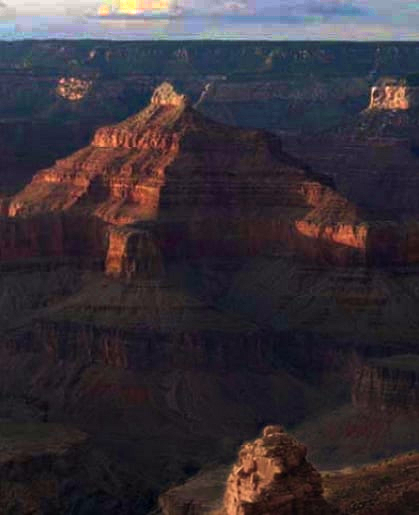
\includegraphics[width=\textwidth]{../dehazed_images/4_dehazed.png}
        \caption{{\scriptsize image désenbrumée du programme}}
        \label{fig:image2}
    \end{subfigure}
    % Troisième image
    \begin{subfigure}[b]{0.27\textwidth}
        \centering
        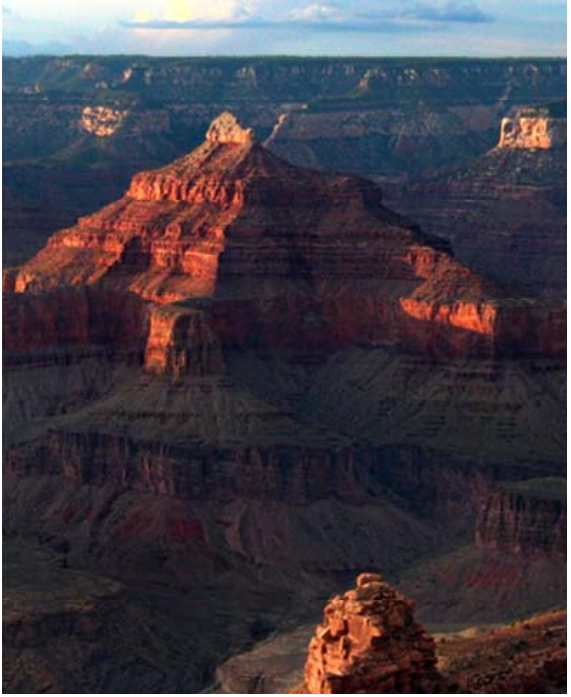
\includegraphics[width=\textwidth]{../thesis_images/4_dehazed.png}
        \caption{{\scriptsize image désenbrumée de la thèse}}
        \label{fig:image2}
    \end{subfigure}
    \caption{Comparaison de l'image obtenue par programme avec l'image de la thèse}
    \label{fig:deux_images}
\end{figure}
Il semble qu'il y ait une meilleure coloration sur l'image fournie par la thèse, mais l'image obtenue par programme reste très semblable : on a l'impression que la brume a été retirée. Les différences doivent résider dans les paramètres qu'on applique à l'algorithme.
\\[1em]
Le principal désavantage de cette méthode est qu'elle est très lente à s'exécuter : elle devient impossible à appliquer sur des grandes images. On est on contraint d'appliquer l'algorithme sur des images de petite résolution (D'où l'apparition de petits carrés sur l'image dans notre programme). Cette contrainte nous amène donc à compresser les images et à en réduire leur qualité. Cela en devient problématique sur certaines images, où beaucoup d'artefacts issus de la compression de l'image altèrent le rendu final.
On a ainsi beaucoup de mal à déterminer la qualité du \textit{dehazer} en se contentant de petites images.

\begin{figure}[H]
    \centering
    % Première image
    \begin{subfigure}[b]{0.27\textwidth}
        \centering
        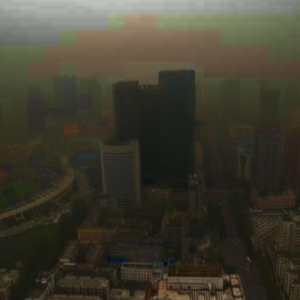
\includegraphics[width=\textwidth]{../dehazed_images/2_crop_dehazed_2.png}
        \caption{{\scriptsize image désembrumée quelconque par notre programme}}
    \end{subfigure}
\end{figure}
\begin{large}
\textbf{Objectifs :}
\end{large}
\\[1em]
Il nous faut absolument rendre l'algorithme bien plus rapide en premier lieu pour avancer dans nos tâches restantes. Il a été conseillé d'implémenter le filtre guidé pour fluidifier les calculs. Ensuite, on doit collecter une base d'images de qualité suffisante pour analyser le comportement et la qualité de la transformation de notre programme. Enfin, il s'agira d'étudier comment le programme se comporte suivant ses paramètres.
\end{document}



